\section{Evaluation}
\label{evaluation}

\subsection{Data set}

Our dataset is the set called \textit{ANN\_IFT1M}\footnote{\url{http://corpus-texmex.irisa.fr/}}. Which is a set of 1,000,000 vectors with dimensionality 128. Vectors are stored as raw little endians. This dataset is created especially for measurements of the approximate nearest neighbour searches.

\subsection{Metrics}

\paragraph{Time} We have three different speed metrics to compare:

\begin{itemize}
  \item Construction time given in milliseconds.
  \item Insertion time given in second.
  \item Query time given in seconds.
\end{itemize}

\paragraph{False negatives} Amount of false negatives for query.
\paragraph{Buckets per partition}

\paragraph{Memory consumption} Total amount of memory needed to create data structure and query it. Given in megabytes and gigabytes.

\subsection{Benchmark}

For measuring our metrics we are using library called \textit{hayai}\footnote{\url{https://github.com/nickbruun/hayai}}, small C++ framework for building benchmarks. It provides toolkit for measuring time, multiple runs and iterations.

\subsection{Test environment}

Experiments were conducted on Intel i5 Processor with 8GB of RAM in 64 bit operating system.

\subsection{Test framework}

Our main idea is to compare and evaluate results of the two LSH implementations - the "covering" and classic one. To do so we first load all data set to our data structure. And then querying them 1500 times for random element. Set of queries is generated upon and same for both sets. The additional overhead is a necessity of having results of each query. By brute force computation we are receiving exact results. Which we can utilize to track false negatives and correctness of received results.

Most important is the radius parameter. Our test cases differs only in radius. Currently we test it against radius of 2,3,4,5. Any higher values requires more superior hardware in terms of memory.

\subsection{Results}

\paragraph{Insertions per second}

Figure ~\ref{fig:insertions-per-second} presents how many insertions per second are performed. As we assumed and can conclude from figure XX  Covering Lsh has lowest performance due need of construction additional buckets. But the gap between Covering Lsh and the regular ones is relatively small and by the radius is increasing we can actually see that the result are coming closer. At the radius of 5 the difference is almost 3 times smaller than at the initial radius of 2. By increasing radius the classic LSH is forced to produce more buckets so one the insertion time increases.

\begin{figure}[ht]
    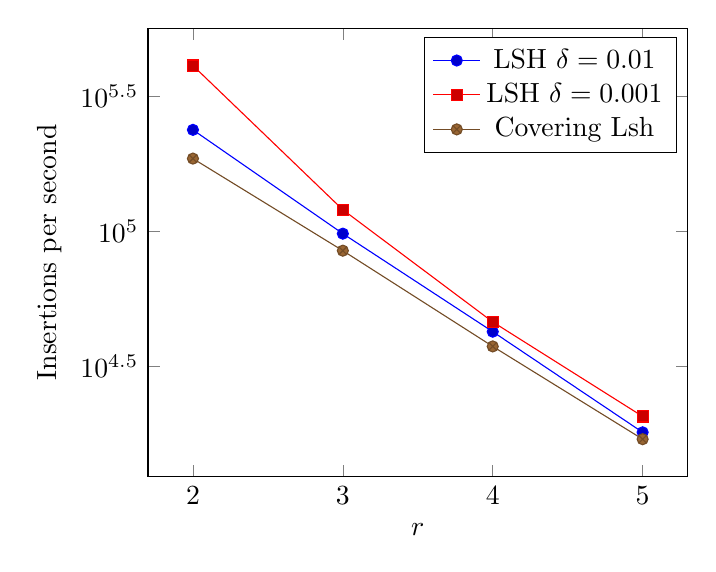
\begin{tikzpicture}
    \begin{semilogyaxis}[
      xlabel = {$r$},
      ylabel = {Insertions per second},
      xtick = data
    ]
      \addplot coordinates {
        (2, 237736.94)
        (3, 98187.51)
        (4, 42593.97)
        (5, 18074.10)
      };

      \addplot coordinates {
        (2, 411106.15)
        (3, 120359.67)
        (4, 46280.57)
        (5, 20693.81)
      };

      \addplot coordinates {
        (2, 186131.05)
        (3, 84934.71)
        (4, 37573.59)
        (5, 17047.07)
      };

      \legend{LSH $\delta = 0.01$, LSH $\delta = 0.001$, Covering Lsh}
    \end{semilogyaxis}
  \end{tikzpicture}

  \caption{Comparision of insertion throughput}
  \label{fig:insertions-per-second}
\end{figure}

\begin{figure}[ht]
  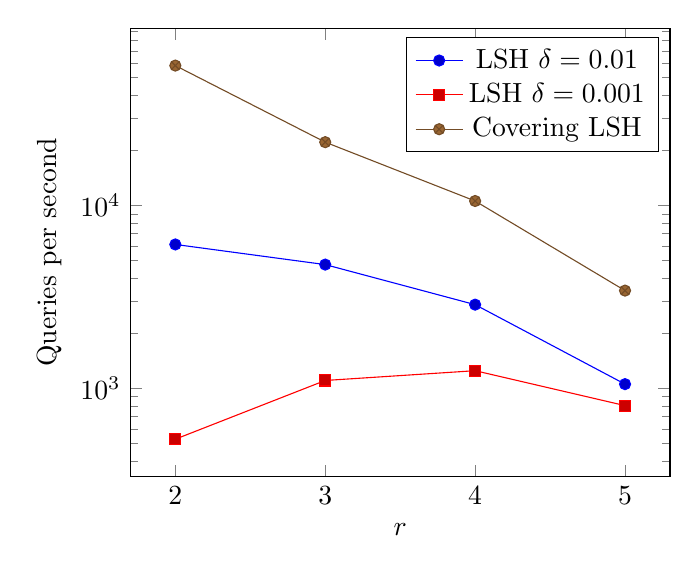
\begin{tikzpicture}
    \begin{semilogyaxis}[
      xlabel = {$r$},
      ylabel = {Queries per second},
      xtick = data
    ]
      \addplot coordinates {
        (2, 6118.88)
        (3, 4747.76)
        (4, 2866.80)
        (5, 1053.48)
      };

      \addplot coordinates {
        (2, 526.67)
        (3, 1103.17)
        (4, 1247.75)
        (5, 803.80)
      };

      \addplot coordinates {
        (2, 58216.55)
        (3, 22187.94)
        (4, 10574.71)
        (5, 3421.63)
      };

      \legend{LSH $\delta = 0.01$, LSH $\delta = 0.001$, Covering LSH}
    \end{semilogyaxis}
  \end{tikzpicture}

  \caption{Comparision of query throughput}
  \label{fig:queries-per-second}
\end{figure}

\paragraph{Buckets per partition}

Figure ~\ref{fig:buckets-per-partition} presents how many buckets per partition is created. This metric show how much Covering Lsh differs from the classic one. Amount of buckets in classic implementations is dependent on the radius. Where the Covering is totally opposite - the buckets count is constant. It is connected to the way how the hash functions family are created [reference]. The trend presented on the plot is very similar to the one from figure ~\ref{fig:insertions-per-second}. Again by increasing the radius the gap is closing. But still the memory overhead is significantly bigger in the Covering that in classic lsh.

\begin{figure}[ht]
  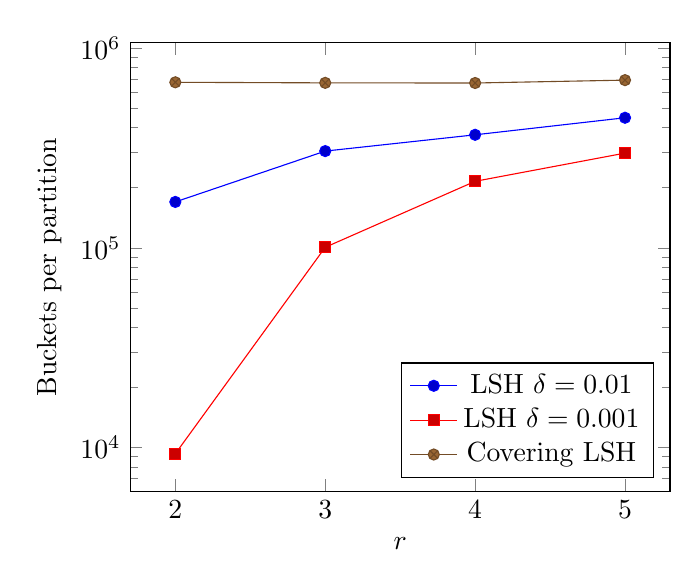
\begin{tikzpicture}
    \begin{semilogyaxis}[
      xlabel = {$r$},
      ylabel = {Buckets per partition},
      xtick = data,
      legend pos = south east
    ]
      \addplot coordinates {
        (2, 169815.43)
        (3, 305179.47)
        (4, 368261.81)
        (5, 448140.33)
      };

      \addplot coordinates {
        (2, 9310.57)
        (3, 100652.33)
        (4, 215357.87)
        (5, 298153.22)
      };

      \addplot coordinates {
        (2, 674554.00)
        (3, 670221.60)
        (4, 669083.68)
        (5, 691636.11)
      };

      \legend{LSH $\delta = 0.01$, LSH $\delta = 0.001$, Covering LSH}
    \end{semilogyaxis}
  \end{tikzpicture}

  \caption{Comparision of bucket distribution}
  \label{fig:buckets-per-partition}
\end{figure}

\paragraph{False negatives per query}

The most important property of the Covering lsh is the fact that it guartees that the queries are not producing false negatives. Figure ~\ref{fig:false-negatives-per-query} show the comparision of this metric between implementations. Obviously the covering holds zero false negatives in each case. More surprising are the results of the classic Lsh. Especially the $\delta = 0.001$ presents very low amount of false negatives across the cases. Next classic lsh is far worse than that; it has more false negatives in each case of $r$.

\begin{figure}[ht]
  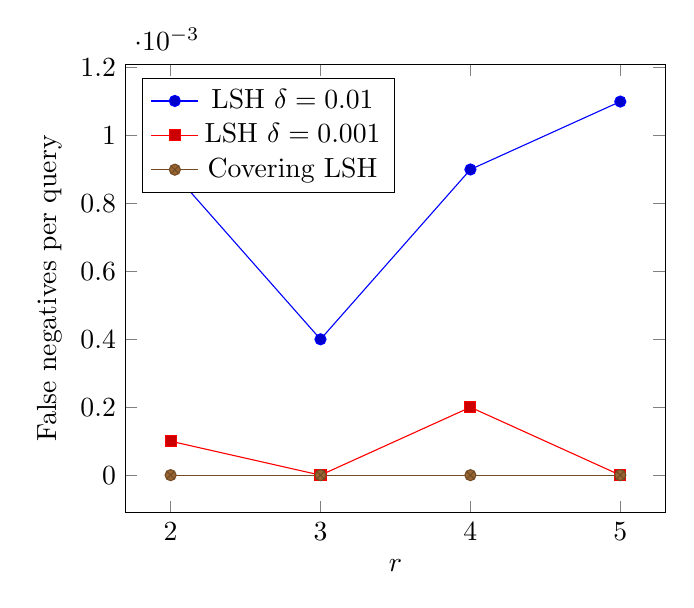
\begin{tikzpicture}
    \begin{axis}[
      xlabel = {$r$},
      ylabel = {False negatives per query},
      xtick = data,
      legend pos = north west
    ]
      \addplot coordinates {
        (2, 0.0009)
        (3, 0.0004)
        (4, 0.0009)
        (5, 0.0011)
      };

      \addplot coordinates {
        (2, 0.0001)
        (3, 0.0000)
        (4, 0.0002)
        (5, 0.0000)
      };

      \addplot coordinates {
        (2, 0.0000)
        (3, 0.0000)
        (4, 0.0000)
        (5, 0.0000)
      };

      \legend{LSH $\delta = 0.01$, LSH $\delta = 0.001$, Covering LSH}
    \end{axis}
  \end{tikzpicture}

  \caption{Comparison of false negative rates}
  \label{fig:false-negatives-per-query}
\end{figure}
